\subsection{Medición entre colector y emisor}


\begin{figure}[h!]
    \centering

    %-------------------------
    %   FIGURA 1
    %-------------------------
    \begin{minipage}[b]{0.40\textwidth}
        \centering
\begin{figure}[H]
    \centering
    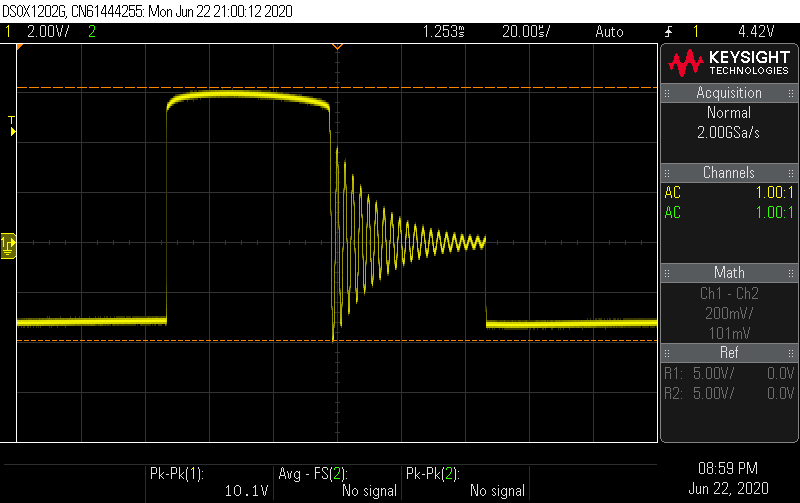
\includegraphics[width=1\textwidth]{imagenes/tp3_f_sinresorte.png}
    \caption{Medición sin resorte usando cable a neutro}
    \label{fig:sinresorte}
\end{figure}

    \end{minipage}
    \hfill
    %-------------------------
    %   FIGURA 2
    %-------------------------
    \begin{minipage}[b]{0.40\textwidth}
        \centering
\begin{figure}[H]
    \centering
    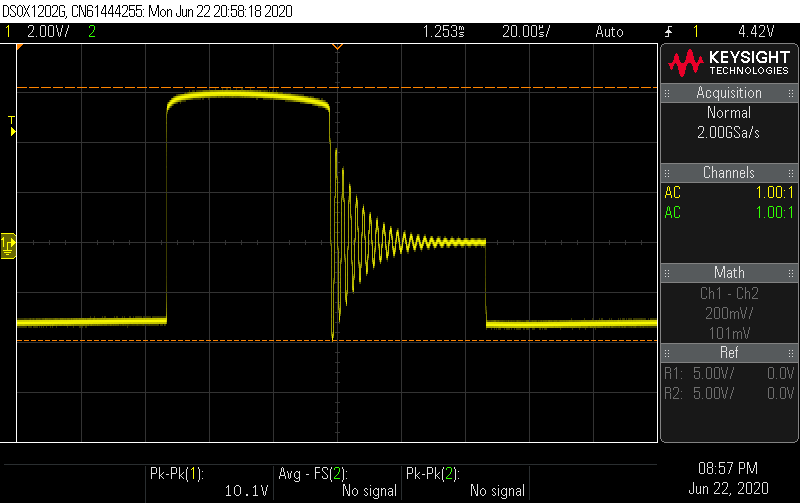
\includegraphics[width=1\textwidth]{imagenes/tp3_f_conresorte.png}
    \caption{Medición con resorte}
    \label{fig:conresorte}
\end{figure}
    \end{minipage}

\end{figure}

En esta parte se midió y comparó la salida entre el emisor y el colector conectando el neutro mediante el cable normal de las puntas del osciloscopio y el accesorio de resorte. El resorte, a diferencia del cable, es una pieza mucho más corta por lo que permite hacer mediciones muchos más precisas. Esto se debe a que al ser más chico, reduce la capacitancia e inductancia parásita al mismo tiempo que reduce el efecto antena que puede causar distorsiones en las mediciones. \par
En particular, al observar las figuras \ref{fig:sinresorte} y \ref{fig:conresorte}, se puede observar que al usar el resorte, el tiempo del transitorio se acorta (Si bien el transitorio se corta antes de terminar, se puede observar una mayor amplitud final en el primero que en el segundo). Esto se puede explicar por la inductancia añadida por el cable y el efecto antena. Al disminuir la longitud del cable, se disminuye la inductancia y el área del lazo que crea el efecto antena, lo que disminuye las tensiones inducidas por el ruido. Estas tensiones parasitas al sumarse al circuito generan, sumado a la inductancia, que el transitorio sea más amplio.